%-----------------------------------------------------------------------------
%
%               Template for sigplanconf LaTeX Class
%
% Name:         sigplanconf-template.tex
%
% Purpose:      A template for sigplanconf.cls, which is a LaTeX 2e class
%               file for SIGPLAN conference proceedings.
%
% Guide:        Refer to "Author's Guide to the ACM SIGPLAN Class,"
%               sigplanconf-guide.pdf
%
% Author:       Paul C. Anagnostopoulos
%               Windfall Software
%               978 371-2316
%               paul@windfall.com
%
% Created:      15 February 2005
%
%-----------------------------------------------------------------------------


%\documentclass[preprint]{sigplanconf}
\documentclass[10pt]{sigplanconf}

% The following \documentclass options may be useful:
%
% 10pt          To set in 10-point type instead of 9-point.
% 11pt          To set in 11-point type instead of 9-point.
% authoryear    To obtain author/year citation style instead of numeric.

\usepackage{yfonts}
\usepackage{amsmath}
\usepackage{amsthm}
\usepackage{amssymb}
%\usepackage{mathpartir}
\usepackage[colorlinks=true,
citecolor=citec,
linkcolor=linkc,
urlcolor=urlc,
]{hyperref}
\usepackage{url}
\usepackage{graphics}
\usepackage{graphicx}
\usepackage{wasysym}
\usepackage{harmony}
\usepackage{marvosym}
\usepackage{multirow}
\usepackage{xspace}
\usepackage[nameinlink,nosort]{cleveref}
\usepackage{xeCJK}
\usepackage[usenames,dvipsnames]{xcolor}
\usepackage[utopia]{mathdesign}
\usepackage{natbib}
\usepackage{ulem}
\usepackage[mathcal]{euscript}
\usepackage[linesnumbered,ruled]{algorithm2e}

\renewcommand{\UrlBreaks}{\do\/\do\a\do\b\do\c\do\d\do\e\do\f\do\g\do\h\do\i\do\j\do\k\do\l\do\m\do\n\do\o\do\p\do\q\do\r\do\s\do\t\do\u\do\v\do\w\do\x\do\y\do\z}


% ____________________________________________________________
% Listings Package Configuration
% \usepackage[scaled]{beramono}

%\renewcommand*\ttdefault{txtt}
\usepackage[T1]{fontenc}

\definecolor{citec}{RGB}{128,0,64}
\definecolor{linkc}{RGB}{0,64,128}
\definecolor{urlc} {RGB}{128,64,0}

\setCJKmainfont{HeiseiMinStd-W5}[Path = ./]
\setmonofont{Inconsolata-Regular}[Path = ./]
% This Deep Tex Voodoo is from
%   <http://www.latex-community.org/forum/viewtopic.php?f=5&t=2072>
% It's purpose is to make \lstinline normal size, without affecting
% \lstinputlisting.  It seems to work but I have no idea how or why,
% and I rather hope never to learn.
%\makeatletter
%\lst@AddToHook{TextStyle}{\let\lst@basicstyle\ttfamily\normalsize}
%\makeatother

\begin{document}

\conferenceinfo{SIGBOVIK '19}{Pittsburgh, PA, USA}
\copyrightyear{2019}
\copyrightdata{}

\titlebanner{banner above paper title}        % These are ignored unless
\preprintfooter{short description of paper}   % 'preprint' option specified.

\title{
Which ITG Stepcharts are Bracket-Jumpiest?: \\
In Which They Milk the \\
「A Boring Follow-Up Paper to \\
``Which ITG Stepcharts are Turniest?'' \\
Titled, ``Which ITG Stepcharts are Crossoveriest and/or Footswitchiest?''」\\
Series for All Its Worth in Publication Count After All, or: \\
%That `Boring' Stuff Was Part of the Title, BTW. \\
%So was that. And that, and this too. \\
%You got it all, right? \\
%Or Just, ``More Boring Crap about ITG'', for Short. \\
%Oh, That Was Also Part of the Title.
Hit Me With An Encore
}
% \subtitle{\em The Randomly-Scoped Lambda Calculus}
% \subtitle{Subtitle Text, if any}

\authorinfo{Ben Blum}{}{bblum@alumni.cmu.edu}

\maketitle

\begin{abstract}
	%ITG is a popular dance game in which players step on arrows while listening to music. The arrow patterns, indicated by a {\em stepchart}, may range among any level of complexity and difficulty. Among the many factors contributing to a stepchart's difficulty is how much the player must turn from side to side.
	%Other more obvious factors, such as raw speed, have been well studied in prior work.
	%This paper presents an analytic study of this {\em turniness} factor.
	%We study the turniness of many existing stepcharts, and present a novel (but unsurprising) approach to automatically generating maximally (or minimally) turny charts.
	%Among real-world songs, we find stepcharts with overall turniness ranging from 0\% to 81.33\% of the theoretical maximum.

In which I break last last year's promise of no future work.

\end{abstract}

\category{D.D.R.}{Exercise and Fitness}{Arcade Dance Games}

\keywords
bracket, groove, in, jumps, the


\section{Introduction}

Recent work by \cite{dril}
%[W. Dril et al., 2019]
proposed the hypothesis that
recent stepchart authors have grown bored with the array of technical ITG step patterns
documented to date \cite{turniness,crossoveriness},
and have moved on to break the old model's one-foot-per-arrow assumption to allow for even more technical patterns yet.
I paraphrase their main conclusion as follows:

\begin{center}
	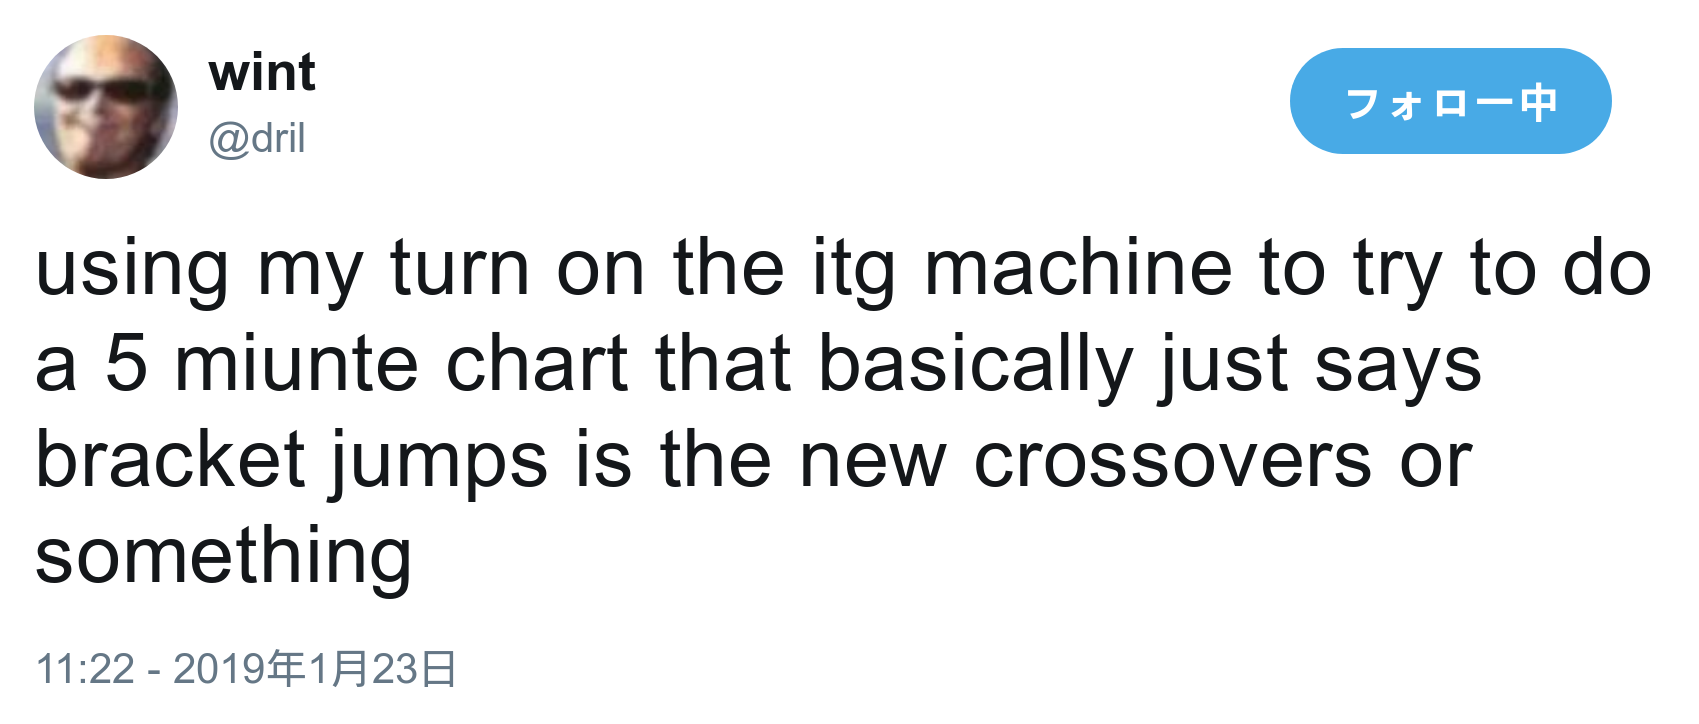
\includegraphics[width=0.38\textwidth]{using-my-turn.png}
\end{center}

\begin{figure}[t]
	\hspace{-2em}\includegraphics[angle=270,width=0.54\textwidth]{../2/paper.pdf}
	\caption{(yeah i reused this joke from last time ok deal)}
	\label{fig:you-stutid-fuckass}
\end{figure}

All good researchers know that when rise the standards for software or hardware performance
(or stepchart trickiness, as the case may be),
they must revisit their own work to prove its ongoing relevance to the research (dance) community at large.
Thus I must regrettably break the promise \sout{I} the authors set forth in \cite{crossoveriness}
(see \Cref{fig:you-stutid-fuckass})
and revisit \sout{my} their old future work section
(XXX: they said to change any first-person ``our prior work''
stuff like this for double-blind review but like cmon this makes no sense?
theyll totally see through this
(TODO: maybe email the PC chair for advice?
(FIXME: make sure to remove these comments before the camera-ready deadline!!))),
extending it to handle these new so-called ``bracket'' jumps.

%%%%%%%%%%%%%%%%%%%%%%%%%%%%%%%%%%%%%%%%%%%%%%%%%%%%%%%%%%%%%%%%%%%%%%%%%%%%%%%%

\section{Overview}

% TODO: go through this paper and make every *other* instance of "bracket-jump" hyphenated

What, then, is a bracket-jump (which I shall \textit{not}, henceforth, abbreviate for brevity)?
Put simply, whenever two arrow-shaped obstacles proceed simultaneously towards the protagonist directional indicator targets
(see \cite{turniness}),
while a novice player might think they must step with both feet at once, one for each arrow,
experts often find it more convenient (i.e., less overall foot motion) to use whichever single foot is closer at the time
to hit both arrows by
triggering one arrow's sensor with the heel and the other with the little bitty toesies.
Pads are typically constructed with a small triangular metal bracket at the corner of each arrow panel,
as shown in \Cref{fig:bracker-detail},
which the bridge of the foot must cross to achieve this, hence the name ``bracket jump''.
In case my prose explanation is not up to snuff, I also show in \Cref{fig:how-2-bracket}
a high-quality graphics render of a player's typical foot positions during a down+right bracket-jump (henceforth ``DR'', et cetera).

The reader, or stepper,
may notice the extreme angle of footing depicted in the latter figure,
which is necessary to reliably trigger both pad sensors.
Accordingly, this maneuver is comfortable (and hence preferable to a normal jump)
only if the player is already facing in roughly the same direction \cite{turniness}.
%after stepping any preceding patterns.
Note also that the two ``candle jumps'', LR and DU, are not possible to bracket,
unless your foot size is (physically) beyond the scope of this work.
The next section will attempt to codify (ahem) when
preceding patterns encourage the player to bracket rather than jump,
and thereby identify how ``bracket jumpy'' each chart is.

\begin{figure}[t]
	\begin{center}
		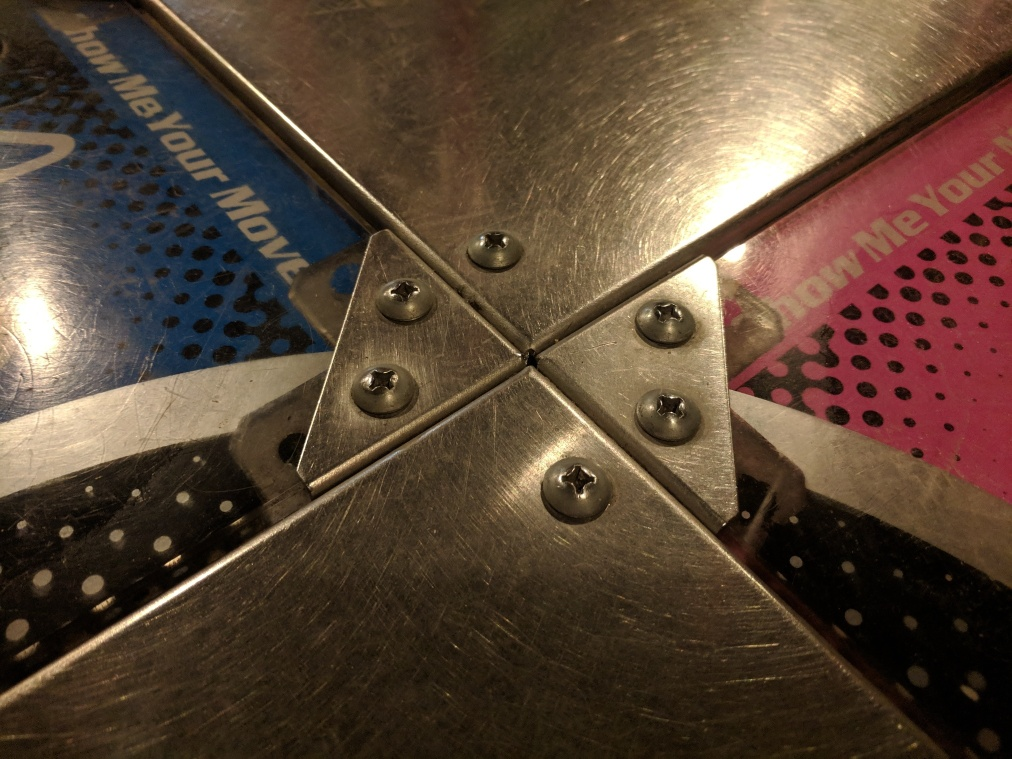
\includegraphics[width=0.48\textwidth]{jims-pix.jpg}
	\end{center}
	\caption{Detail of metal corner brackets, this paper's namesake. Photo credit {\tt JIM}.}
	\label{fig:bracker-detail}
\end{figure}

\begin{figure}[h]
	\begin{center}
		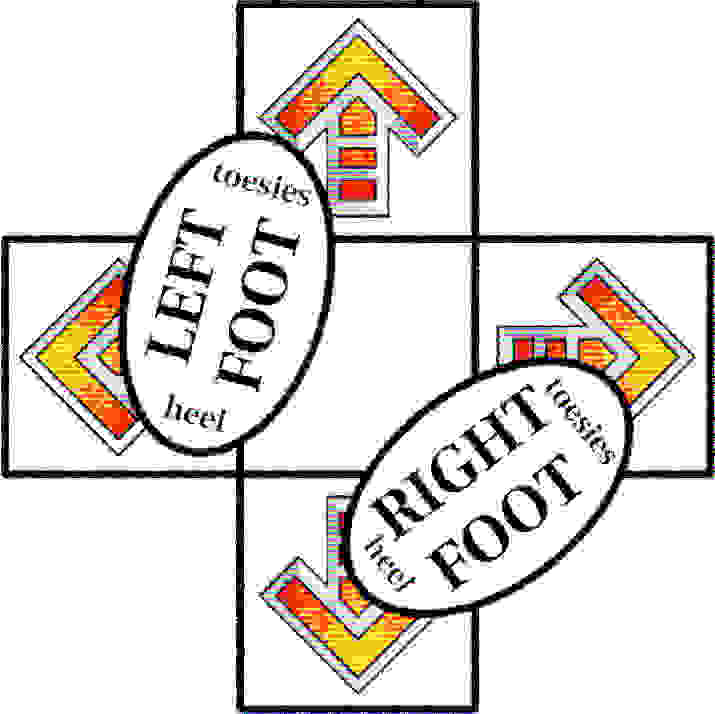
\includegraphics[width=0.3625\textwidth]{how-2-bracket.jpg}
	\end{center}
	\caption{Down+right bracket-jump real-world example.}
	\label{fig:how-2-bracket}
\end{figure}

%%%%%%%%%%%%%%%%%%%%%%%%%%%%%%%%%%%%%%%%%%%%%%%%%%%%%%%%%%%%%%%%%%%%%%%%%%%%%%%%

\section{Algorithm Design}
\label{sec:analyzing}

I extended the crossoveriness et cetera algorithm from \cite{crossoveriness} to reason about jumps,
which previously it treated all identically,
ignoring the arrows involved and allowing the player to reset her footing as desired.
Now, it considers LD, LU, DR, and UR jumps as potentially bracketable,
allowing the player to continue a stream of alternating feet uninterrupted through.

\textit{Confession.}
When I was first brainstorming this project,
I had some grand visions of unifying the turniness algorithm \cite{turniness}---which
accounts for U/D steps to figure out how far the player must turn each step,
but has no idea which way she is actually facing at any given time---with
the crossoveriness one
(cited just above; cmon how much do you want me to repeat these same two citations, gimme a break)---which
totally ignores U/D steps and just figures out which arrows the left and right feet must each step---in
some theoretically beautiful way to produce the unquestionably perfect footing sequence for each jump.
%
However, as I was considering how to incorporate features from last time's algorithm,
potentially allowing crossover brackets (\Cref{sec:xover-brackers})
and footswitch brackets (\Cref{sec:fs-brackers}),
I realized that ultimately there would be no restrictions on what jumps were bracketable;
the algorithm would oops simply twist and turn as much as necessary to bracket everything,
and this paper would become just ``Which ITG Stepcharts Have the Most Jumps?'', and like who wants to read that.

One may think to simply try either bracketing each jump or not
and seeing what combination gives the minimum turniness result,
but since whether to bracket each jump or not affects subsequent steps' footing,
each choice cannot in general be solved independently,
and I hope you can see where this is going.
Now, the last time I tried to solve an exponentially-sized problem, it took me 7 years
\cite{landslide-thesis}
(and I still ended up with a pile of heuristics after all anyway),
so considering I started this project a week before the deadline,
I opted instead to just code up a bunch of ad-hoc rules to handle all the different bracket jump patterns
that occurred to me to write test cases for.

As before, the code is available at \url{https://github.com/bblum/sigbovik/blob/master/itg/code/ITG.hs}.
To give a sense of how much its elegance has been despoiled % hi william
since the last version:
62 lines of Haskell (which computed crossovers, footswitches, jacks, doublesteps, \textit{and} crossover footswitches)
has grown to 156 lines (just to handle this one. new. feature),
and the once-simple datatype definition of

\newcommand\hilight[2]{\color{#1}#2\color{black}\xspace}
\definecolor{pink}{RGB}{128,0,192}
\definecolor{orange}{RGB}{192,96,0}
\definecolor{olivegreen}{RGB}{0,127,32}
\definecolor{brickred}{RGB}{192,0,0}
\definecolor{commentblue}{RGB}{0,128,192}

\begin{center}
	\texttt{\hilight{orange}{data}~\hilight{olivegreen}{Step} =
	\hilight{brickred}{L} |
	\hilight{brickred}{D} |
	\hilight{brickred}{U} |
	\hilight{brickred}{R} |
	\hilight{brickred}{Jump}}
\end{center}

has become the unwieldy:

\vspace{-1em} % dont know why this is necessary
\begin{center}
	\begin{tabular}{l}
	\texttt{\hilight{orange}{data}~\hilight{olivegreen}{Arrow} =
	\hilight{brickred}{L} |
	\hilight{brickred}{D} |
	\hilight{brickred}{U} |
	\hilight{brickred}{R}} \\
	\texttt{\hilight{orange}{data}~\hilight{olivegreen}{Jump} =
	\hilight{brickred}{LD} |
	\hilight{brickred}{LU} |
	\hilight{brickred}{DR} |
	\hilight{brickred}{UR} |
	\hilight{brickred}{LR} |
	\hilight{brickred}{DU} |
	\hilight{brickred}{Other}} \\
	\texttt{\hilight{orange}{data}~\hilight{olivegreen}{Step} =
	\hilight{brickred}{A} \hilight{olivegreen}{Arrow} |
	\hilight{brickred}{J} \hilight{olivegreen}{Jump}} \\
	\texttt{\hilight{orange}{data}~\hilight{olivegreen}{Foot} =
	\hilight{brickred}{LeftFoot} |
	\hilight{brickred}{RightFoot}} \\
	\end{tabular}
\end{center}

The general gist is that in addition to tracking which foot stepped the last arrow and optimizing for alternating feet,
we also track which arrow(s) each foot was last on,
and whenever we encounter a LD/LU/DR/UR jump, bracket it if both:
\begin{enumerate}
	\item The last foot is opposite the foot required for the jump (e.g. L for LD), and
	\item The last foot's last note(s) does not intersect the arrows involved in the jump (i.e., R not on D preceding LD).
\end{enumerate}
In lieu of a detailed algorithm listing, I'll simply show some of those most notable test cases in pictures and explain in prose how the implementation must handle them,
which was pretty much my implementation strategy to begin with.

\Cref{fig:tests} shows a bunch of patterns with a bracketable jump,
and each subfigure in \Cref{fig:tests2} shows a corresponding unbracketable case.
%with a similar pattern.
Whenever two jumps are pictured in the same unit test, we are concerned with whether the latter one is bracketable.
I'll now explain how the algorithm handles each case.

\begin{figure}[t]
	\begin{center}
	\begin{tabular}{ccc}
		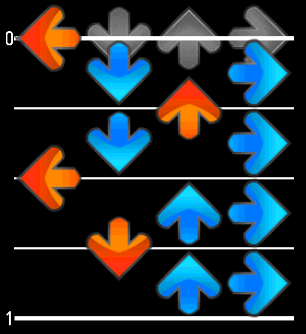
\includegraphics[width=0.14\textwidth]{test-basic-yes.png} & 
		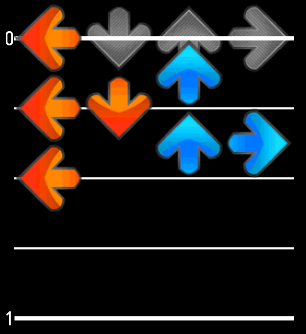
\includegraphics[width=0.14\textwidth]{test-footswitch-bracket-yes.png} &
		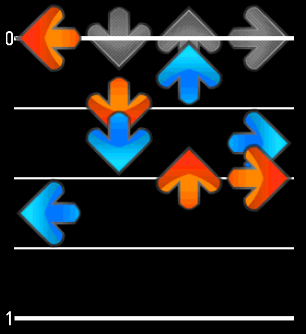
\includegraphics[width=0.14\textwidth]{test-reset-footing-yes.png} \\
		(a) All 4 OK
		&
		(b) LD, UR OK
		&
		(c) UR OK
		\\
		\\
		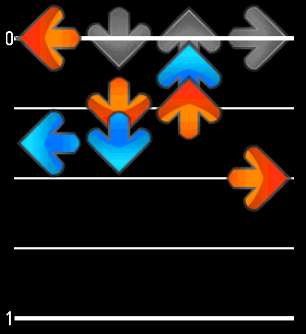
\includegraphics[width=0.14\textwidth]{test-propagate-through-ud-yes.png} &
		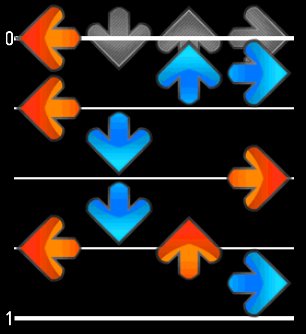
\includegraphics[width=0.14\textwidth]{test-reset-subsequent-stream-yes.png} &
		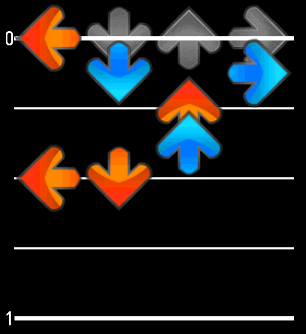
\includegraphics[width=0.14\textwidth]{test-footswitch-jack-yes.png} \\
		(d) LD OK
		&
		(e) UR, LU OK
		&
		(f) DR, LD OK
	\end{tabular}
	\end{center}
	\caption{Examples of bracketable jumps.}
	\label{fig:tests}
\end{figure}
\begin{figure}[t]
	\begin{center}
	\begin{tabular}{ccc}
		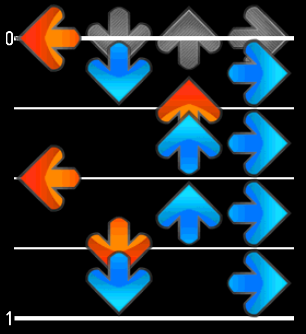
\includegraphics[width=0.14\textwidth]{test-basic-no.png} &
		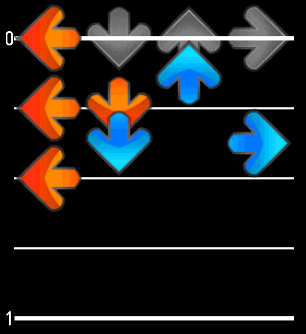
\includegraphics[width=0.14\textwidth]{test-footswitch-bracket-no.png} &
		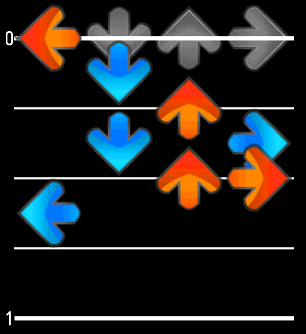
\includegraphics[width=0.14\textwidth]{test-reset-footing-no.png} \\
		(a) 2nd, 4th NG
		&
		(b) DR NG
		&
		(c) UR NG
		\\
		\\
		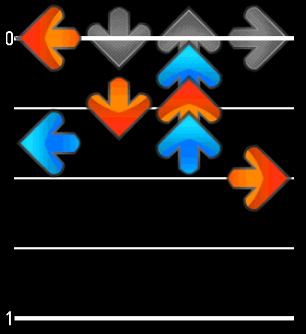
\includegraphics[width=0.14\textwidth]{test-propagate-through-ud-no.png} &
		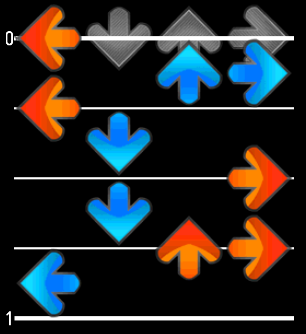
\includegraphics[width=0.14\textwidth]{test-reset-subsequent-stream-no.png} &
		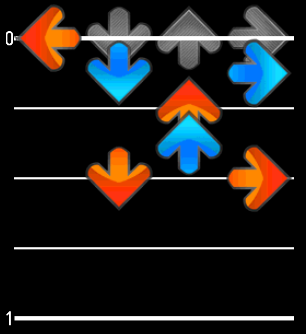
\includegraphics[width=0.14\textwidth]{test-footswitch-jack-also-yes.png} \\
		(d) LU NG
		&
		(e) 2nd UR NG
		&
		(f) Trick question
	\end{tabular}
	\end{center}
	\caption{Examples of unbracketable jumps,
	each corresponding to the similar pattern in \Cref{fig:tests}.}
	\label{fig:tests2}
\end{figure}

\renewcommand{\theenumi}{\alph{enumi}}
\begin{enumerate}
	\item In the OK case, the right foot can bracket every jump (condition 1),
		as the left foot is always on a different arrow than the jump (condition 2).
		In the NG case, condition 2 is violated for the second and fourth jumps.
	\item Version of (a) testing that preceding bracket-jumps also contribute to condition 2.
		The NG case would be a footswitch bracket requiring rather uncomfortable footing angles.
	\item In OK, LR cannot be bracketed, but clears the prior footings so UR can.
		In NG, LR can be bracketed, meaning UR cannot while still alternating feet (condition 1).
	\item DU jumps can never be bracketed, but can be stepped facing either direction, and this must respect prior footings.
		In both cases DU is stepped with right foot U, which allows bracketing LD but not LU thereafter.
	\item In OK, the crossover does not interfere with either bracket and the player can alternate feet throughout.
		In NG, either doublestepping or jumping normally is required
		(or a future-work crossover bracket; see \Cref{sec:xover-brackers}).
	\item In OK, the player easily footswitches on U.
		In the corresponding case, the player can actually just jack U instead, stepping it twice with her left foot
		before bracketing DR again with her right.
\end{enumerate}
\renewcommand{\theenumi}{\arabic{enumi}}

These examples are available as {\tt test-bracket-*.sm} unit tests in the code repository.
Hopefully armed with this understanding of the bracket jumping rules, let's now move on to real-world stepcharts.

% non bracket jumps reset the lastarrowLR

% no footswitch bracket - angles of yr ankles hurt
% propagate thru UD
% tiebreak preceding stream
% retroactively cancel if last stream hadta switch

%%%%%%%%%%%%%%%%%%%%%%%%%%%%%%%%%%%%%%%%%%%%%%%%%%%%%%%%%%%%%%%%%%%%%%%%%%%%%%%%

\section{Evaluation}

The experimental corpus has grown even more since last time, now comprising %17253
17340 % with ups 4
stepcharts from 182 packs.
Of note, all three Technical Showcase packs
(collaborative packs where the community at large was encouraged to submit their freshest beats and judged on complexity)
were released in the last two years,
which have proved to be important sources of diverse bracket-jump patterns for this research.
I would also have liked to re-rank the crossoveriest and footswitchiest charts from last time to include these submissions,
but I frankly don't have time.
The results spreadsheet of bracket jump counts
(as well as more crossovers, footswitches, et cetera for charts newer than the last paper)
is available for your browsing pleasure at
\url{https://tinyurl.com/bracketiest}.

% command used to generate the sheet
% used "|" as sed delimiter bc others appear in song names
% IFS=$'\n'; for i in `find ~/stepmania/Songs/ | grep '\.sm$'`; do cat "$i" | ./ITG 2>&1 | sed "s|^|$i\t|"; done > ../3/results/results.txt

I pose two evaluation questions, to be answered in the following subsections respectively.
\begin{enumerate}
	\item Which songs, packs, and/or step-cartographers are bracket-jumpiest?
	\item Is bracket jumps the new crossovers or something?
\end{enumerate}

\subsection{Bracket-Jumpiness}
\label{sec:bjness}

I measured the overal bracketiness of each chart in two ways,
first,
by comparing the number of bracket jumps against the total number of steps,
or the \textit{bracket-jump step percentage} (BJS\%);
second,
by comparing against the total number of jumps only,
or the \textit{bracket jump jump percentage} (BJJ\%).
The BJS\% indicates a chart's overall density of steps requiring the player to step across the brackets
(which depends on how jumpy the chart is to begin with),
whereas the BJJ\% measures perhaps the author's intentionality in patterning their jumps either as brackets,
or as random where just some of them happen to be bracketable.

\Cref{tab:bjs} shows the leaderboard for the former metric, and \Cref{tab:bjj} the latter.%
\footnote{When measuring BJJ\% I excluded charts with fewer than 10 jumps in total,
which put up a handful of false positives in the 100\% ranks.}
Note that the aforementioned recent Technical Showcase pack series put up three bracketiest charts in the BJJ\% category;
meanwhile, the UPS packs, known for their gimmicks and general lack of respect for player comfort,
secure several top spots on the BJS\% board.
For comparison's sake, the overall BJJ\% of the entire corpus is 19.8\% (93k/470k),
meaning that roughly 1 in 5 randomly-patterned jumps are by chance bracketable.
The overall BJS\% (a thoroughly less meaningful statistic) is 0.7\%.

\begin{table}[t]
	\begin{center}
		\small
	\begin{tabular}{r|l|l|r|r}
		\bf Ft. & \bf Name & \bf Pack & \bf \#BJ & \bf BJS\% \\
		\hline
		10 & SOBA			& Squeaky Beds \&c.	& 366 & 83\% \\
		11 & Get Off of My Way		& UPS 3			& 115 & 28\% \\
		12 & Hardware Store		& Keyboard Coll. III	& 207 & 23\% \\
		13 & Firestorm			& BemaniBeats 3		& 153 & 31\% \\
		14 & Bounce			& UPS 2			& 126 & 21\% \\
		15 & Ikaros Dynamite!!!!	& UPS 2			& 238 & 34\% \\
		16 & Mermaid Island		& Tachyon Alpha		& 346 & 49\% \\
		17 & Toccata \& Fugue		& CuoReNeRo M.P.	& 255 & 24\% \\
		% this chart is ALL jumps so it's kinda false positive
		%420 & Paa			& UPS 4			& 263 & 34\% \\
	\end{tabular}
	\end{center}
	\caption{Charts of each difficulty with the highest bracket-jump density among all steps (BJS\%).}
	\label{tab:bjs}
\end{table}
\begin{table}[t]
	\begin{center}
		\small
	\begin{tabular}{r|l|l|r|r}
		\bf Ft. & \bf Name & \bf Pack & \bf \#BJ & \bf BJJ\% \\
		\hline
		 9 & Drifting Away		& UPS 4			&  26 &  88\% \\
		10 & SOBA			& Squeaky Beds \&c.	& 366 &  99\% \\
		11 & Save Miracles		& ECFA 2019		&  42 &  95\% \\
		12 & Electrical Paradise	& Chic. Timing Auth.	&  35 & 100\% \\
		12 & Encore			& Tech. Showcase	&  29 & 100\% \\
		12 & Nemeton			& Subluminal		&  12 & 100\% \\
		13 & Decadent Dandy		& Tech. Showcase 3	&  12 & 100\% \\
		14 & Nageki no Ki		& Valex's M.4-A.A. 8	& 116 &  94\% \\
		15 & Beach Party		& Tech. Showcase 2	& 162 &  80\% \\
		16 & Mermaid Island		& Tachyon Alpha		& 346 &  79\% \\
		17 & Zombie Sunset		& Jummy Jawns 2		& 325 &  88\% \\
		69 & koopa bling		& UPS 4			&  39 &  98\% \\
	\end{tabular}
	\end{center}
	\caption{Charts of each difficulty with the highest percentage of their total jumps bracketable (BJJ\%).
	All participants of the 3-way tie for 12-footers are listed.}
	%filtered by having at least 10 jumps to begin with.}
	\label{tab:bjj}
\end{table}

Next up is bracket jumpiness by pack and by author.
\Cref{tab:pack-bjs,tab:pack-bjj} show the top 10 packs in both bracketiness metrics,
and \Cref{tab:author-bjs,tab:author-bjj} the top 10 authors
(filtered by having written at least 10 charts).
For the packs, I also list the release year of each;
note how despite the relatively even spread of years in BJS\%,
2018 dominates the BJJ\% leaderboard,
suggesting that older charts' bracket-jumps arose by chance simply from having a lot of jumps to begin with.
I'll come back to this point in \Cref{sec:eval-years}.
In honorable mentionth place is chart author Halogen-, whose 11 charts contain 154 jumps, \textit{none} of which are bracketable.
What a purist!

\begin{table}[t]
	\begin{center}
		\small
	\begin{tabular}{l|r|r|r}
		\bf Pack name & \bf Year & \bf \#charts & \bf BJS\% \\
		\hline
		Keyboard Collaboration III		& $\le$2012	&  17 & 12.4\% \\
		Squeaky Beds and Leaky Faucets		& 2018	& 125 &  4.9\% \\
		Keyboard Collaboration I		& $\le$2012	&  12 &  3.6\% \\
		CuoReNeRo MeGaPacK			& N/A	& 460 &  3.3\% \\
		Mute Sims X2 WIP			& 2018	&  12 &  3.0\% \\
		r2112					& 2007	&  60 &  2.7\% \\
		Technical Showcase 3			& 2018	& 196 &  2.7\% \\
		FoxyMix 4 - Nuclear Overdrive		& $\le$2012	&  67 &  2.6\% \\
		Technical Showcase 2			& 2017	&  80 &  2.6\% \\
		Gensokyo Midnight			& $\le$2012 	&  77 &  2.5\% \\
	\end{tabular}
	\end{center}
	\caption{Song packs densest in bracket jumps.}
	\label{tab:pack-bjs}
\end{table}

% sorry about my sigfig discrepancies between this and the by-chart table but like, latex and margins yknow
\begin{table}[t]
	\begin{center}
		\small
	\begin{tabular}{l|r|r|r}
		\bf Pack name & \bf Year & \bf \#charts & \bf BJJ\% \\
		\hline
		Feelin' Rusty 3			& 2018	&  51 & 50.2\% \\
		Squeaky Beds and Leaky Faucets	& 2018	& 125 & 46.7\% \\
		TYLR's Technical Difficulties	& 2018	&  33 & 44.9\% \\
		Technical Showcase 3		& 2018	& 196 & 41.7\% \\
		Mute Sims X2 WIP		& 2018	&  12 & 40.9\% \\
		Jimmy Jawns 2			& 2015	&  55 & 39.7\% \\
		Technical Showcase 2		& 2017	&  80 & 38.2\% \\
		Keyboard Collaboration III	& $\le$2012	&  17 & 38.1\% \\
		Chicago Timing Authority	& 2018	&  33 & 36.3\% \\
		DVogan's Tech Support 2		& 2018	&  32 & 36.1\% \\
	\end{tabular}
	\end{center}
	\caption{Song packs with the most jumps bracketable.}
	\label{tab:pack-bjj}
\end{table}

\subsection{Historical Trends}
\label{sec:eval-years}

I sought to prove \cite{dril}'s claim that bracket-jumps have skyrocketed in popularity in the most recent years of stepchart-making,
%I decided to do this
by finding the progression of bracketiness across past years of stepchart packs.
However,
actually assigning a firm release date to every pack on my hard drive turned out to be a feat of internet archaeology unto itself,
even involving archive.org for one step.
I'll spare you the details, but you can peruse them in the second spreadsheet of the dataset linked at the start of this section.
Ultimately, all packs older than 2013 had to be grouped together,
as no pack collection website, facebook group, or laptop filesystem could accurately date enough packs
before then to give meaningful sample sizes for each year.
I also decided to exclude tournament packs such as ECFA from this analysis,
which curate existing stepcharts written possibly long ago.

\textit{Statistical significance.}
Stepcharts thus dated, I then summed the total steps, jumps, and brackets published in each year,
and analyzed the resulting overall BJS\% and BJJ\% as a linear regression.
\Cref{fig:stats} shows the best-fit and 95\% confidence intervals,
plotted in R \cite{r-lang} with ggplot \cite{ggplot}.
For BJS\%, the $\le$2012 bucket actually produced the highest data point (at 11.8\%);
I suspect this simply represents the fact that jumps were more popular overall during ITG's nascency
(as corroborated by \Cref{tab:pack-bjs}).
Owing to this and also to its nature as an aggregation over nearly a decade (which spoils the linear model anyway),
I chose to exclude it from BJS\%,
but keep it for BJJ\%, which overall jump count has no bearing on.
(Its linear fit has $\beta$ = 0.012\%, CI = \{-0.08,+0.10\}, not significant.)
For the two pictured distributions, their confidence intervals do not include 0,
i.e., a flat line representing no growth,
so I conclude bracket jumps' increased popularity is statistically significant.

\begin{table}[t]
	\begin{center}
		\small
	\begin{tabular}{l|r|r}
		\bf Author name & \bf \#charts & \bf BJS\% \\
		\hline
		Paul J Kim & 45 & 9.9 \\
		sssmsm & 45 & 4.4 \\
		Liam & 11 & 3.4 \\
		Snooze & 22 & 2.5 \\
		M. Emirzian & 26 & 2.2 \\
		bblum & 40 & 1.9 \\
		Ninevolt & 10 & 1.7 \\
		B. Vergara & 95 & 1.6 \\
		C. Emirzian & 18 & 1.6 \\
		B. Dinh & 10 & 1.6 \\
		Renard & 51 & 1.5 \\
	\end{tabular}
	\end{center}
	\caption{Step cartographers who write charts densest in bracket-jumps.}
	\label{tab:author-bjs}
\end{table}

\begin{table}[t]
	\begin{center}
		\small
	\begin{tabular}{l|r|r}
		\bf Author name & \bf \#charts & \bf BJJ\% \\
		\hline
		Paul J Kim & 45 & 71.8 \\
		Rust & 97 & 51.7 \\
		bblum & 40 & 49.3 \\
		Liam & 11 & 44.5 \\
		Snooze & 22 & 38.1 \\
		Rems & 10 & 36.5 \\
		sssmsm & 45 & 32.9 \\
		Loak & 19 & 31.7 \\
		Little Matt & 42 & 31.4 \\
		Paparazzi & 10 & 29.6 \\
	\end{tabular}
	\end{center}
	\caption{Step cartographers whose jumps are most bracketable.}
	\label{tab:author-bjj}
\end{table}

%% more sigfigs values provided
% the 95% CI for step (excluding <=2012) is _(0.032,0.139)_
% the 95% CI for jump (including all years) is _(0.396,2.208)_
% step (not all years): 0.085
% jump: 1.302
% step (all years): 0.012 with a 95% CI of (-0.080, 0.104) (edited)

%%%% ggplot code provided by neuropantser
% # set up data vectors
% bracket_jump = 100*c(0.1816545127,0.1614241831,0.1486753945,0.1755102041,0.1593747466,0.2210173322,0.2676218299,0.2333917477)
% year_jump = 2012:2019
% 
% bracket_step = 100*c(0.005698341736,0.003965042926,0.00499281212,0.005327880519,0.006349085019,0.007480904624,0.01087723206)
% year_step = 2013:2019
% 
% # run linear models (and manually output the 95% CIs)
% step_lin = summary(lm(bracket_step~year_step))
% print(sprintf("95 pct CI for step: (%s,%s)",step_lin$coefficients[2,1]-1.96*step_lin$coefficients[2,2],
%               step_lin$coefficients[2,1]+1.96*step_lin$coefficients[2,2]))
% jump_lin = summary(lm(bracket_jump~year_jump))
% print(sprintf("95 pct CI for jump: (%s,%s)",jump_lin$coefficients[2,1]-1.96*jump_lin$coefficients[2,2],
%               jump_lin$coefficients[2,1]+1.96*jump_lin$coefficients[2,2]))
% 
% # plot the linear trends
% library(ggplot2)
% 
% # directory to store plots -- CHANGE THIS to where you want them stored
% plotdir = "C:/Users/mtlawson/Pictures/stuff"
% 
% # create temp dataset with bracket_jump variables
% plotdata = data.frame(year_jump,bracket_jump)
% # construct plot
% jump = (ggplot()
%         + geom_point(data=plotdata,aes(x=year_jump,y=bracket_jump),alpha=0.7,col='red')
%         + geom_smooth(data=plotdata,aes(x=year_jump,y=bracket_jump),method='lm',alpha=0.4)
%         + xlab("Year")
%         + ylab("Brackets-Vs-Jumps Pct")
%         + scale_x_continuous(breaks=year_jump)
%         + theme_classic())
% # output to pdf (can switch to PNG or other desired filetype)
% pdf(file=sprintf("%s/jump_plot.pdf",plotdir))
% print(jump)
% dev.off()
% # create temp dataset with bracket_step variables
% plotdata = data.frame(year_step,bracket_step)
% # construct plot
% step = (ggplot()
%         + geom_point(data=plotdata,aes(x=year,y=bracket_step),alpha=0.7,col='red')
%         + geom_smooth(data=plotdata,aes(x=year,y=bracket_step),method='lm',alpha=0.4)
%         + xlab("Year")
%         + ylab("Brackets-Vs-Steps Pct")
%         + scale_x_continuous(breaks=year_step)
%         + theme_classic())
% # output to pdf (can switch to PNG or other desired filetype)
% pdf(file=sprintf("%s/step_plot.pdf",plotdir))
% print(step)
% dev.off()

\begin{figure}[t]
	\begin{tabular}{c}
		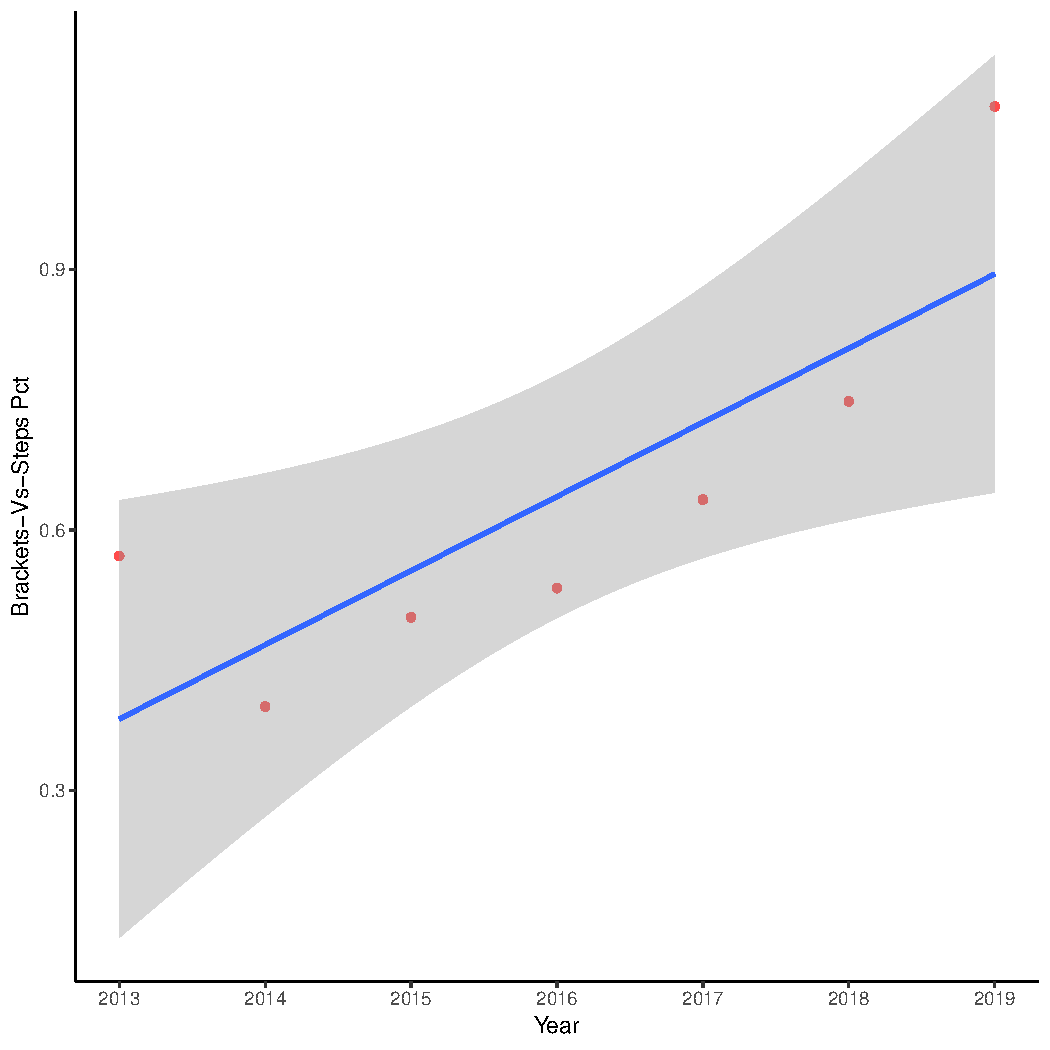
\includegraphics[width=0.42\textwidth]{step_plot.pdf}
		\\
		(a) BJS\% across years ($\beta$ = 0.085\%/yr, CI = \{0.032,0.14\}).
		\\
		\\
		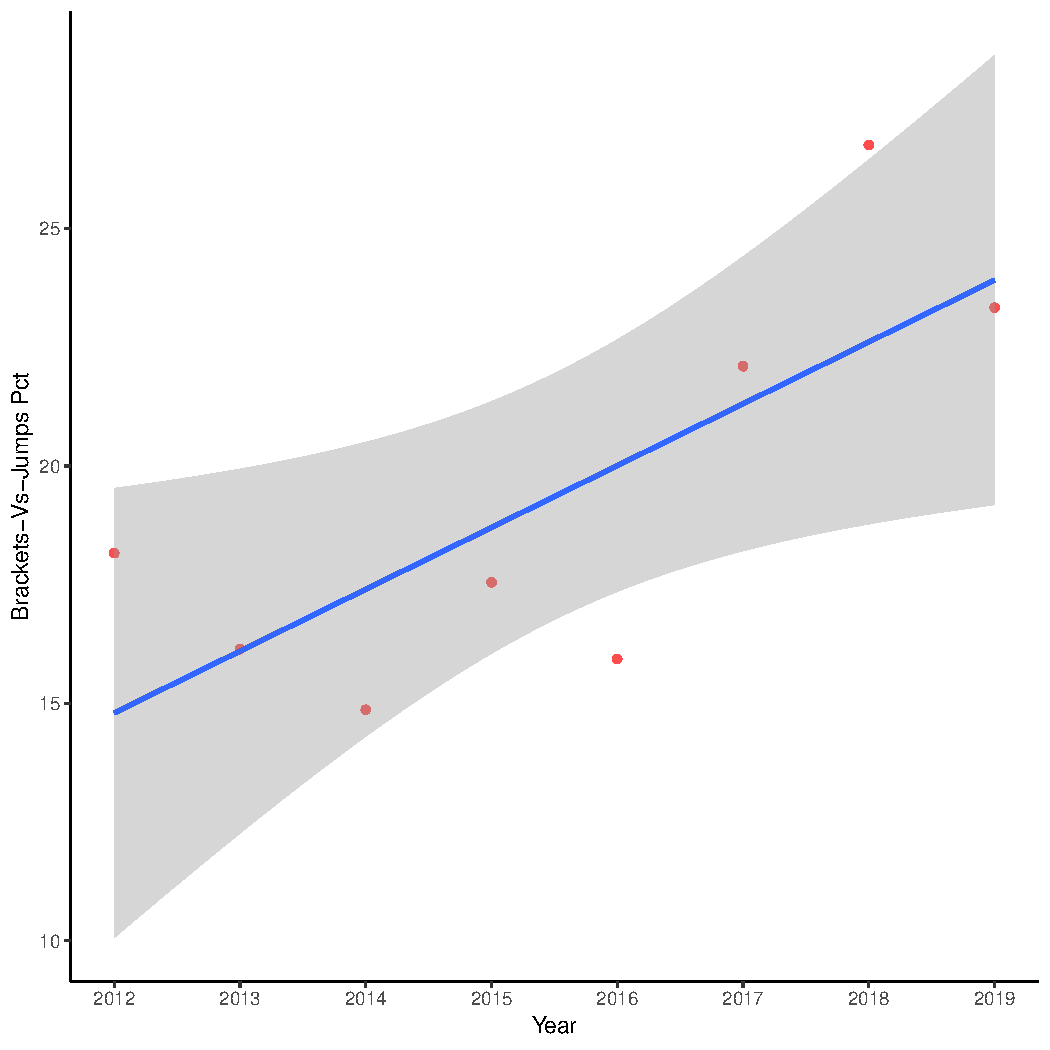
\includegraphics[width=0.42\textwidth]{jump_plot.pdf}
		\\
		(a) BJJ\% across years ($\beta$ = 1.30\%/yr, CI = \{0.40,2.21\}).
	\end{tabular}
	\caption{Linear best fit of bracket jumps' popularity across the years of ITG's history.
	Grey area depicts 95\% CI.}
	\label{fig:stats}
\end{figure}

\textit{Bias.}
This analysis is prone to selection bias in my own pack downloading habits:
supposing I suddenly became more interested in playing brackety charts recently,
that would certainly influence how many bracket-jumps appeared each year in this corpus.
However, I believe the BJJ\% measurement adequately compensates for this,
for if I suddenly became interested in stamina instead of technical and added a bunch of 10-minute trance packs,
that would impact only BJS\%.
As far as I know, I show no preference for more or less jumpy charts overall than the community average,
leading me to trust the BJJ\% test.

%%%%%%%%%%%%%%%%%%%%%%%%%%%%%%%%%%%%%%%%%%%%%%%%%%%%%%%%%%%%%%%%%%%%%%%%%%%%%%%%

\section{Discussion}

% TODO: check figure placement
\begin{figure*}[t]
	\begin{center}
	\begin{tabular}{c}
		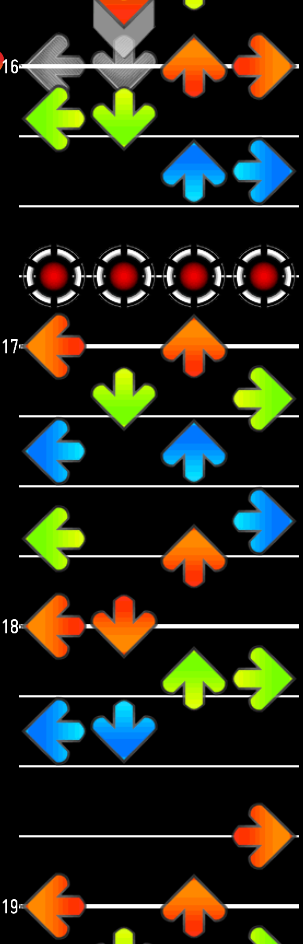
\includegraphics[width=0.16\textwidth]{disco-beachparty.png}
		\\
		(a) Beach Party, \\ 15 \cite{beachparty} %\\
	\end{tabular}
	\begin{tabular}{c}
		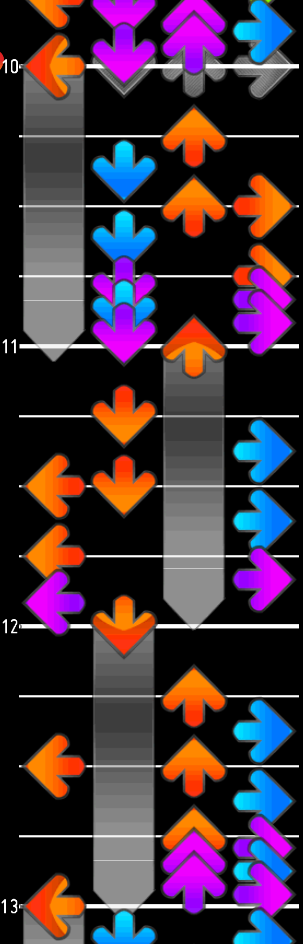
\includegraphics[width=0.16\textwidth]{disco-koopa.png}
		\\
		(b) koopa bling, \\ 69 \cite{koopa} %\\
	\end{tabular}
	\begin{tabular}{c}
		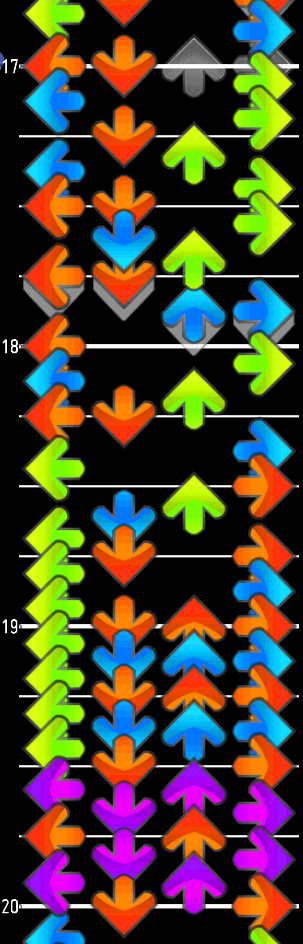
\includegraphics[width=0.16\textwidth]{disco-zombiesunet.png}
		\\
		(c) Zombie Sunset, \\ 17 \cite{zombie} %\\
	\end{tabular}
	\begin{tabular}{c}
		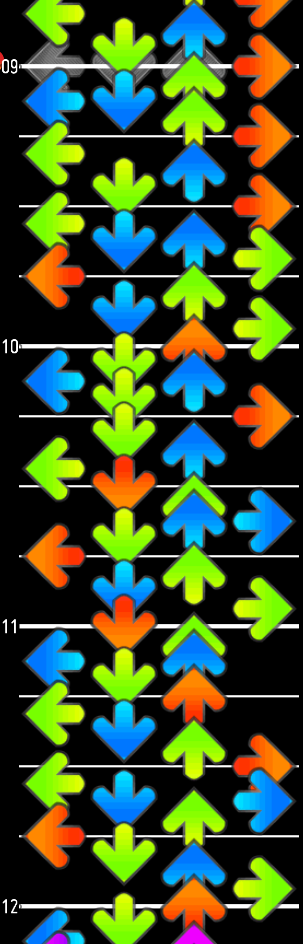
\includegraphics[width=0.16\textwidth]{disco-owa.png}
		\\
		(d) 1-Winged Angel, \\ 14 \cite{owa} %\\
	\end{tabular}
	\begin{tabular}{c}
		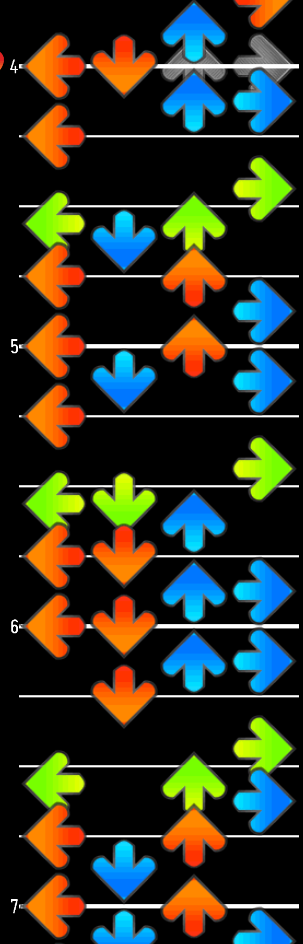
\includegraphics[width=0.16\textwidth]{disco-paradise.png}
		\\
		(e) Electrical Paradise, \\ 12 \cite{e-paradise} %\\
	\end{tabular}
	\end{center}
	%\caption{Why I gotta write a overall caption, just read the prose on this one.}
	\caption{Example real-world charts with
	(a) false negative jumps that mines render bracketable after all,
	(b) jumps whose footing is affected by preceding holds fixing one foot in place,
	%false negative jumps forced to bracket by preceding holds, % XXX: this is a lie!! bonus pts if anyone spots it. i don't actually know why the alg didn't classify
	(c) brackets the chart author was sorry about,
	(d) ``retro'' style unbracketable jump-stream, %which, largely, cannot be bracketed,
	and
	(e) intentionally many true bracket jumps from the BJJ\% category winner.}
	\label{fig:discussion}
\end{figure*}

I confirmed in stepmania the bracketiness of each of \Cref{sec:bjness}'s high scorers,
and happily observed no false positives (i.e., all charts seemed to intend the player to bracket),
surprising myself for the 3rd time running at the accuracy of the algorithm.
I did observe some false negatives, i.e., jumps seeming intended to be bracketed that the algorithm wouldn't catch.
In Beach Party \cite{beachparty}, shown in \Cref{fig:discussion}(a),
the ``mine jump'' forces the player to reset her footing,
removing the right foot's initial presence on U to allow LU to be bracketed.
This would actually be pretty easy to fix (just have the algorithm parse mines like, at all)
but it's the day of the deadline and I already ran the experiment, so.
Another class of false positives showed up in koopa bling \cite{koopa} (\Cref{fig:discussion}(b)),
where one foot is fixed to a hold, affecting the footing of subsequent jumps.%
\footnote{The algorithm actually foots them correctly in this chart by sheer luck (an even number of preceding doublesteps maintains footing parity),
but these would be harder to handle in general.}
For kicks, I also show the source of the ``I'm sorry'' stepchart description in \Cref{fig:discussion}(c),
from Zombie Sunset \cite{zombie} (\Cref{tab:bjj});
note here the DUR bracket-triple-jumps in the third measure,
which the algorithm currently cannot process.

Many old charts written without regard to jump patterning allow for many of their jumps to be bracketed anyway.
I noticed an old stepchart for One-Winged Angel \cite{owa} ranking high in the list of overall total bracket-jumps,
with 182,
simply because it's long and has a lot of steps,
but upon playing, the patterns definitely do not feel intentional,
and it even includes a section of stream with wholly unbracketable jumps interspersed.
\Cref{fig:discussion}(d) shows this section;
in this stream, the player would expect to step the red and blue arrows with her right foot and the lime ones with her left,
but note how the jumps (hint: all in blue arrows, unless you're reading this on dead trees)
occur as a mix of left and right arrows, with even a UD ``candle'' jump making an appearance.
However, it measures an unremarkable 9 BJS\% and 38 BJJ\%---I just wanted to feature it
as an example of what non-bracketable jump stream looks like.

Authors seem to realize when their charts are too bracket jumpy for comfort:
several of the charts appearing in the highest ranks of the spreadsheet had their step author field filled in as ``Stupid'' or ``I'm sorry''.
In fact, I personally found the charts with 100 BJJ\%, i.e., \textit{all} jumps appearing therein were bracketable,
to be more tasteful than those with more total BJS\% but a few normal jumps as well.
I'd hypothesize this is because to achieve 100 BJJ\% requires a certain intentionality,
resulting in better chart design overall
(note that such charts necessarily include no LR or DU jumps whatsoever).
Either that, or the more uncomfortable ones include certain extremely turny/candley/doublesteppy patterns
around their brackets that causes the algorithm to count them as normal jumps instead.
Anyway, \Cref{fig:discussion}(e) shows the chart with most bracket-jumps (35) among ones with 100 BJJ\%,
which I tried out for myself and found quite enjoyable \cite{e-paradise}.
Amusingly, Encore \cite{encore}
features a Hard chart in addition to its Challenge,
which former ranks second place to Electrical Paradise among 100 BJJ\%s with 29 brackets.
Upon inspection, I found this chart identical to the Challenge (upcoming in \Cref{fig:xb}(a)),
only the crossover brackets
(to be discussed later in \Cref{sec:xover-brackers})
having been replaced by easier, normal ones.

\section{Never Work}

The only thing that impresses the research community more than overdelivering on your future work promises
is to overdeliver twice; hence, I shamelessly reuse the joke of this section name from last time.

\subsection{UI}

It would be cool to integrate this (and the preceding two algorithms \cite{turniness,crossoveriness})
into
%Simply Love \cite{simplylove}, or whatever
the community's prevailing stepmania theme.
%may be in the future.
Currently, as shown in \Cref{fig:songpreview}(a),
the song preview screen wastes considerable space displaying the count of irrelevant chart aspects
such as mines (now used primarily for signaling the presence of footswitches)
and hands (now mostly stepped with the feet by bracketing anyways).
I bet the community might actually pay attention to my work---the holy grail of research, honestly---if
popular themes used it to show precisely how technical a chart was, as in (b).

\begin{figure}[t]
	\begin{tabular}{c}
	
\includegraphics[width=0.46\textwidth]{song-info.png} \\
		(a) Current state-of-the-art.
		\\
		\\
	
\includegraphics[width=0.46\textwidth]{song-info-better.png} \\
		(b) Artist's conception.
	\end{tabular}
	\caption{Song info preview panel for a recent bracket jump-heavy stepchart \cite{divine}.}
	\label{fig:songpreview}
\end{figure}

\subsection{Crossover Brackets}
\label{sec:xover-brackers}

Whereas with normal crossovers (e.g., in the sequence L-U-R, stepping the R with the left foot),
the player's foot can pretty much point whichever way she finds most comfortable;
however,
crossover brackets (e.g., in the sequence L-U-DR...),
the player's foot must point backwards (...stepping the DR's R with her left heel and D with toes),
inducing extra turniness.%
\footnote{The other way, e.g. stepping the D with the left heel and R with toes, while your right foot is fixed on U, is extremely uncomfortable at speed. Trust me on this one.}
Such jumps could instead just be stepped with both feet as normal,
possibly inducing doublesteps or jacks,
and indeed that is how the algorithm presently handles them.

However, ambitious stepchart authors have recently experimented with encouraging the player to bracket-jumps while crossed-over.
Such charts attempt to force, or at least hint, these jumps to be bracketed
via additional stepchart elements: in \Cref{fig:xb}(a), mines on the left arrow force the player to remove her left foot in preparation for the crossover (and being in the middle of fast stream, further discourages doublestepping),
and in \Cref{fig:xb}(b), extending one of the arrows as a hold encourages the player to bracket the subsequent jump with the other foot.
In (b)'s case, the player must also switch feet on each of the non-hold arrows,
effectively making these crossover-footswitch-brackets,
which would truly be a wonder to identify programmatically.
% these can be cheated anyway
Note however the high measure counter in both, meaning these occur quite late in the song;
both charts first spend some time ``teaching'' the player both to expect bracket jumps
and how it intends to signal crossovers in general---so if a human is not expected to understand them at first glance,
I think it is fair to leave out of the algorithm too for now.

\begin{figure}[t]
	\begin{center}
	\begin{tabular}{cc}
	\begin{tabular}{c}
		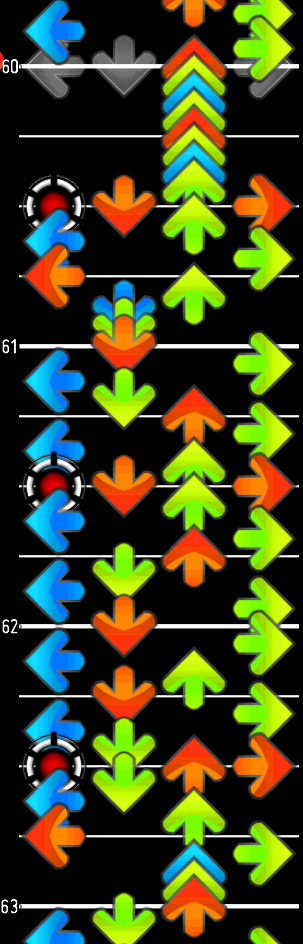
\includegraphics[width=0.16\textwidth]{xb-encore.png}
		\\
		(a) Encore, 12 \\ \cite{encore} %\\
		%(12, Tech. Showcase 1)
	\end{tabular}
		&
	\begin{tabular}{c}
		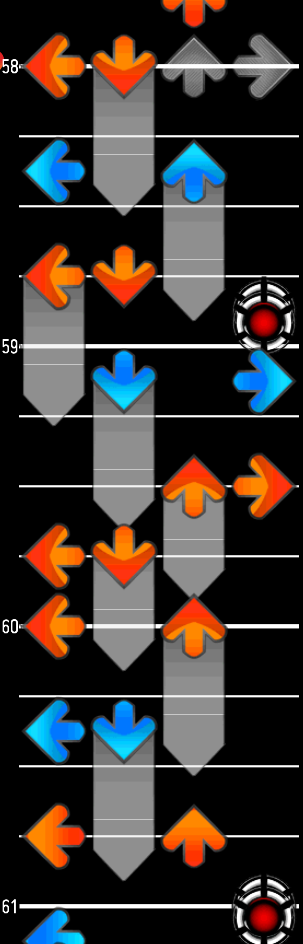
\includegraphics[width=0.16\textwidth]{xb-atariwave.png}
		\\
		(a) Atariwave, 10 \\ \cite{atariwave} %\\
		%(10, Tech. Showcase 3)
	\end{tabular}
	\end{tabular}
	\end{center}
	\caption{Crossover bracket-jumps must be signaled via either (a) mines or (b) holds to remove ambiguity.}
	\label{fig:xb}
\end{figure}

\subsection{Footswitch Brackets}
\label{sec:fs-brackers}

I put this section here only just so I could have something to forward-reference back in \Cref{sec:analyzing},
but not to actually write anything.
I always wanted to do that, you know?
I mean, footswitch brackets are %also
a real thing, but still. $\bar{~~}$\textbackslash\_(ツ)\_/$\bar{~~}$
% not-to-to: put a pict anyway? if you find one
% actually, joke comes off better w/o

\subsection{Obligatory Machine Learning Section}

I guess you could skip all this fiddly ``algorithm'' stuff by
hopping on the pads yourself for a few rounds, playing a variety of technical charts,
and just training a neural network based on how you stepped the patterns.
It would probably even learn to fake crossovers more at the ends of songs than at the beginnings,
where you're more likely to be physically tired.
And like, do you really want that kind of bias in your dataset?

Remember kids, friends don't let friends use ML for problems that are more fun to solve by hand.

\section{Conclusion}

Bracket jumps is, in fact, statistically significantly, the new crossovers or something.
%I never know what to put down here. Much love to the community..!

\acks

neuropantser (Michael T. Lawson) provided invaluable eleventh-hour (literally) advice
on \Cref{sec:eval-years}'s statistical analysis, up to and including making the graphs for me.
Greg Hanneman unknowingly helped copy-edit my hyphenation.
And much love to the SIGBOVIK community.

%%%%%%%%%%%%%%%%%%%%%%%%%%%%%%%%%%%%%%%%%%%%%%%%%%%%%%%%%%%%%%%%%%%%%%%%%%%%%%%%

\bibliographystyle{abbrvnat}
\bibliography{citations}

\end{document}
